\apendice{Especificación de diseño}

\section{Introducción}
Este apéndice detalla la arquitectura interna del sistema SugAIr y las decisiones de diseño tomadas durante su desarrollo. El objetivo es proporcionar una visión técnica clara sobre cómo se estructuran e interactúan los distintos componentes de \textit{software} que conforman la plataforma. Al tratarse de un sistema centrado en la Inteligencia Artificial y la privacidad, la arquitectura difiere de las aplicaciones móviles tradicionales basadas en la nube, adoptando un enfoque de procesamiento local y sin persistencia de datos tradicional.

\section{Diseño de datos}
Dada la naturaleza del proyecto y el requisito fundamental de Privacidad por Diseño, el sistema SugAIr carece de una base de datos persistente (como SQL o NoSQL). No se almacena historial de conversaciones, perfiles de usuario ni telemetría. El diseño de datos se centra exclusivamente en las estructuras de intercambio de información en memoria, utilizando el formato JSON para la comunicación entre capas.

Para estandarizar este intercambio, la API REST se ha diseñado siguiendo la especificación OpenAPI (versión 3.0.3). Las estructuras de datos principales son las siguientes:

\begin{itemize}
    \item \textbf{Objeto de Petición (\texttt{ChatRequest}):} Estructura enviada desde la aplicación móvil al servidor. Contiene dos propiedades de tipo texto (\textit{string}): \texttt{content} (el mensaje del usuario) e \texttt{image} (la fotografía codificada en Base64, de carácter opcional).
    \item \textbf{Objeto de Respuesta (\texttt{ChatResponse}):} Estructura devuelta por el servidor a la aplicación móvil. Contiene una única propiedad de tipo texto llamada \texttt{message}, que incluye la respuesta generada por la IA.
    \item \textbf{Objeto de Inferencia (\texttt{OllamaRequest}):} Estructura interna generada por el servidor backend para comunicarse con el motor local. Incluye el nombre del modelo (\texttt{model}: \textit{llava-diabetes}), el parámetro \texttt{stream} (configurado en \textit{false} para respuestas síncronas) y la matriz de imágenes.
\end{itemize}

\section{Diseño arquitectónico}
El sistema SugAIr se ha diseñado siguiendo un patrón arquitectónico Cliente-Servidor estructurado en \textbf{tres capas lógicas}. Esta separación de responsabilidades facilita el escalado de componentes de \textit{software} independientes y garantiza que el pesado procesamiento de los modelos de IA no sature la interfaz. En la figura \ref{fig:arquitectura} se ilustra el diagrama de componentes lógicos de la plataforma.

\begin{figure}[htbp]
    \centering
    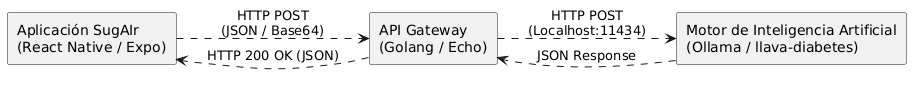
\includegraphics[width=1\linewidth]{arquitectura_sugair.png}
    \caption{Diagrama de arquitectura lógica del sistema SugAIr.}
    \label{fig:arquitectura}
\end{figure}

\subsection{Capa de Presentación (Frontend)}
Constituye el punto de interacción directo con el usuario final. Está implementada como una aplicación móvil multiplataforma desarrollada con \textbf{React Native} y el entorno de herramientas de \textbf{Expo}. Es responsable de renderizar la interfaz de usuario, gestionar el estado dinámico de la conversación, acceder a las APIs nativas del dispositivo (galería de imágenes) y aplicar la compresión inicial de las fotografías.

\subsection{Capa Lógica (API Gateway)}
Actúa como un puente seguro y un orquestador de peticiones. Está desarrollada en \textbf{Golang} haciendo uso del \textit{framework} de enrutamiento rápido \textbf{Echo}. Recibe las peticiones de la aplicación móvil en el puerto 8080 y gestiona el enrutamiento bidireccional hacia el motor local, transformando los datos al formato específico requerido y controlando los tiempos de espera (\textit{timeouts}).

\subsection{Capa de Inferencia}
SugAIr emplea un motor de inferencia local impulsado por \textbf{Ollama}. Es el encargado de alojar en memoria y ejecutar el modelo de lenguaje multimodal \texttt{llava-diabetes}. Decodifica las imágenes en Base64, analiza el texto del usuario aplicando la comprensión del contexto clínico y genera la respuesta final.

\section{Diseño procedimental}
El diseño procedimental define la lógica interna y el flujo algorítmico que sigue el sistema para resolver una tarea. En SugAIr, el procedimiento principal es el ciclo de envío y recepción de un mensaje. 

El algoritmo implementado en la aplicación móvil (\texttt{index.tsx}) y en el servidor (\texttt{main.go}) sigue el siguiente flujo de ejecución síncrono:

\begin{enumerate}
    \item \textbf{Validación de entrada:} La interfaz bloquea el envío si el campo de texto está vacío y no hay una imagen adjunta. Si hay imagen, se extrae de la galería y se comprime directamente a Base64 puro.
    \item \textbf{Bloqueo de interfaz:} Se activa el estado de carga (\textit{loading}) mostrando un indicador visual (\texttt{ActivityIndicator}) y deshabilitando temporalmente el botón de envío.
    \item \textbf{Petición de red:} El cliente formatea la petición HTTP \texttt{POST} hacia \texttt{/api/v1/chat} utilizando la librería \textit{Axios} y queda a la espera.
    \item \textbf{Orquestación (\textit{Backend}):} El servidor en Go recibe la petición, extrae el cuerpo JSON y construye una nueva petición dirigida a la API interna de Ollama (\texttt{localhost:11434}).
    \item \textbf{Inferencia:} El modelo \texttt{llava-diabetes} procesa la información y devuelve la respuesta.
    \item \textbf{Resolución y renderizado:} El servidor Go recibe la respuesta de Ollama, comprueba que el código HTTP sea 200 (OK) y se la devuelve al cliente móvil. La interfaz desactiva el estado de carga, inyecta la nueva respuesta en el contenedor de mensajes de la pantalla y restablece los controles. En caso de error de red o estado HTTP anómalo, la lógica captura la excepción e imprime un mensaje de error visualizado en color rojo.
\end{enumerate}
\begin{comment}
    
\apendice{Especificación de diseño}

\section{Introducción}

\section{Diseño de datos}

\section{Diseño arquitectónico}

\section{Diseño procedimental}

\end{comment}


